%! TEX root = ../thesis.tex
\section{Experimental Results}
\label{kks:sec:eval}

\begin{figure}
	\centering
	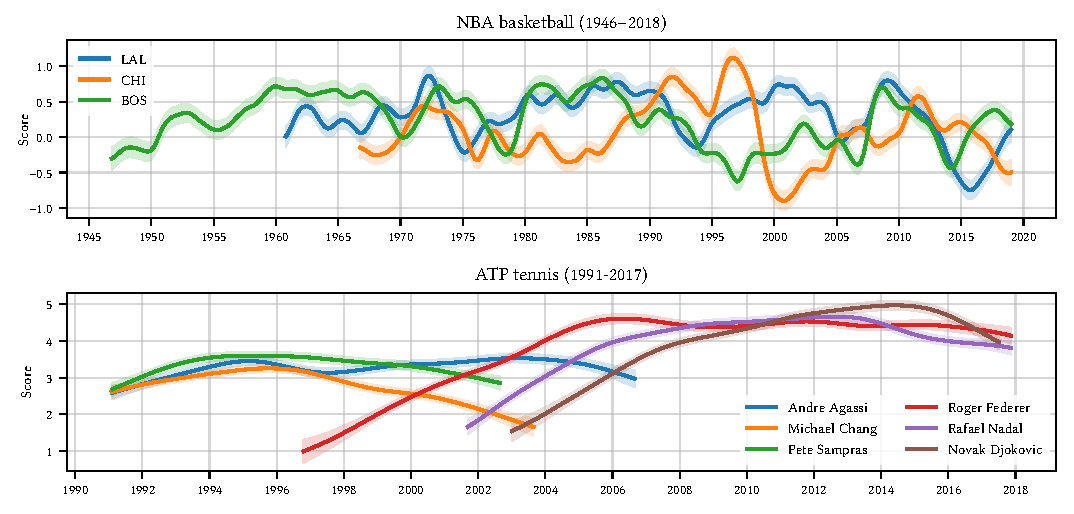
\includegraphics[width=\textwidth]{kks-scores}
	\caption{
		Temporal evolution of the score processes ($\mu \pm \sigma$) corresponding to selected basketball teams (top) and tennis players (bottom).
		The basketball teams are the Los Angeles Lakers (LAL), the Chicago Bulls (CHI) and the Boston Celtics (BOS).}
	\label{kks:fig:scores}
\end{figure}

% Introduction to the section.
In this section, we evaluate our model and inference algorithm on real data.
Our experiments cover three aspects.
First, in Section~\ref{kks:sec:evaldyn}, we compare the predictive performance of our model against competing approaches, focusing on the impact of flexible time-dynamics.
Second, in Section~\ref{kks:sec:evalgen}, we show that by carefully choosing features and observation likelihoods, predictive performance can be improved significantly.
Finally, in Section~\ref{kks:sec:evalinf}, we study various facets of our inference algorithm.
We measure the impact of the mean-field assumption and of the choice of variational objective, and we demonstrate the scalability of the algorithm.

\paragraph{Datasets}
We consider six datasets of pairwise-comparison outcomes of various sports and games.
Four of them contain timestamped outcomes; they relate to tennis, basketball, association football and chess.
Due to the large size of the chess dataset\footnote{%
	This dataset consists of all the match outcomes contained in \emph{ChessBase Big Database 2018}, available at \url{https://shop.chessbase.com/en/products/big_database_2018}.}, we also consider a subset of the data spanning 30 years.
The two remaining datasets contain match outcomes of the StarCraft computer game and do not have timestamps.
Table~\ref{kks:tab:datasets} provides summary statistics for all the datasets.
Except for chess, all data are publicly available online\footnote{%
	Tennis: \url{https://github.com/JeffSackmann/tennis_atp},
	basketball: \url{https://projects.fivethirtyeight.com/nba-model/nba_elo.csv},
	football: \url{https://int.soccerway.com/},
	StarCraft: \url{https://github.com/csinpi/blade_chest}.
}.

\begin{table}
	\centering
	\caption{
		Summary statistics of the sports datasets.}
	\label{kks:tab:datasets}
	\sisetup{table-text-alignment=right}
	\begin{tabular}{l lS[table-format=6.0]S[table-format=7.0]l}
		\toprule
		Name            & Ties & $M$    & $N$     & Time span  \\
		\midrule
		ATP tennis      & No   & 20046  & 618934  & 1991--2017 \\
		NBA basketball  & No   & 102    & 67642   & 1946--2018 \\
		World football  & Yes  & 235    & 19158   & 1908--2018 \\
		ChessBase small & Yes  & 19788  & 306764  & 1950--1980 \\
		ChessBase full  & Yes  & 343668 & 7169202 & 1475--2017 \\
		\addlinespace
		StarCraft WoL   & No   & 4381   & 61657   & ---        \\
		StarCraft HotS  & No   & 2287   & 28582   & ---        \\
		\bottomrule
	\end{tabular}
\end{table}

\paragraph{Performance Metrics}
Let $(\bm{x}, t^*, y)$ be an observation.
We measure performance by using
the logarithmic loss: $-\log p(y \mid \bm{x}, t^*)$ and
the accuracy: $\Indic{y = \Argmax_{y'} p(y' \mid \bm{x}, t^*)}$.
We report their average values on the test set.

\paragraph{Methodology}
Unless specified otherwise, we partition every dataset into a training set containing the first 70\% of the observations and a test set containing the remaining 30\%, in chronological order.
The various hyperparameters (such as covariance functions and their parameters, learning rates, etc.) are selected based on the training data only, by maximizing the log-marginal likelihood of Bayesian models and by minimizing the average leave-one-out log loss otherwise.
% The final hyperparameter configuration of all models can be found in Appendix~\ref{app:eval}.
In order to predict the outcome of an observation at time $t^*$, we use \emph{all} the data (in both training and test sets) up to the day preceding $t^*$.
This closely mimics the setting where a predictor must guess the outcome of an event in the near future based on all past data.
Unless specified otherwise, we use Algorithm~\ref{alg:inference} with the EP variational objective, and we declare convergence when the improvement in log-marginal likelihood falls below $10^{-3}$.
Typically, the algorithm converges in less than a hundred iterations.


%%%%%%%%%%%%%%%%%%%%%%%%%%%%%%%%%%%
\subsection{Flexible Time-Dynamics}
\label{kks:sec:evaldyn}

% Description of the experiment
In this experiment, we compare the predictive performance of our model against competing approaches on four timestamped datasets.
In order to better isolate and understand the impact of accurately modeling \emph{time dynamics} on predictive performance, we keep the remaining modeling choices simple: we treat all outcomes as ordinal-valued (i.e., \emph{win}, \emph{loss} and possibly \emph{tie}) with a probit likelihood and use a one-to-one mapping between competitors and features.
In Table~\ref{kks:tab:predperf}, we report results for the following models:
\begin{itemize}
	\item \emph{Random}. This baseline assigns equal probability to every outcome.

	\item \emph{Constant}. The model of Section~\ref{kks:sec:model} with a constant covariance function.
	      This model assumes that the scores do not vary over time.

	\item \emph{Elo}. The system used by the World Chess Federation~\citep{elo1978rating}.
	      Time dynamics are a by-product of the update rule (c.f. Section~\ref{kks:sec:relwork}).

	\item \emph{TrueSkill}. The Bayesian model of~\citet{herbrich2006trueskill}.
	      Time dynamics are assumed to follow Brownian motion (akin to our Wiener kernel) and inference is done in a single pass over the data.

	\item \emph{Ours}. The model of Section~\ref{kks:sec:model}.
	      We try multiple covariance functions and report the one that maximizes the log-marginal likelihood.
\end{itemize}

\begin{sidewaystable}
	\centering
	\caption{
		Predictive performance of our model and of competing approaches on four datasets, in terms of average log loss and average accuracy.
		The best result is indicated in bold.}
	\label{kks:tab:predperf}
	\sisetup{table-format=1.3, detect-all}
	\begin{tabular}{l SS SS SS SS SSl}
		\toprule
		                & \multicolumn{2}{c}{Random}    & \multicolumn{2}{c}{Constant} & \multicolumn{2}{c}{Elo}
		                & \multicolumn{2}{c}{TrueSkill} & \multicolumn{3}{c}{Ours}                                                                                       \\
		\cmidrule(r){2-3}               \cmidrule(r){4-5}               \cmidrule(r){6-7}
		\cmidrule(r){8-9}               \cmidrule{10-12}
		Dataset         & Loss                          & \text{Acc.}                  & Loss                    & \text{Acc.}     & Loss                  & \text{Acc.}
		                & Loss                          & \text{Acc.}                  & Loss                    & \text{Acc.}     & Covariance                          \\
		\midrule
		ATP tennis      & 0.693                         & 0.500                        & 0.581                   & 0.689           & 0.563                 & 0.705
		                & 0.563                         & 0.705                        & \bfseries 0.552         & \bfseries 0.714 & Affine + Wiener                     \\
		NBA basketball  & 0.693                         & 0.500                        & 0.692                   & 0.536           & 0.634                 & 0.644
		                & 0.634                         & 0.644                        & \bfseries 0.630         & \bfseries 0.645 & Constant + Matérn 1/2               \\
		World football  & 1.099                         & 0.333                        & 0.929                   & \bfseries 0.558 & 0.950                 & 0.551
		                & 0.937                         & 0.554                        & \bfseries 0.926         & \bfseries 0.558 & Constant + Matérn 1/2               \\
		ChessBase small & 1.099                         & 0.333                        & 1.030                   & \bfseries 0.478 & 1.035                 & 0.447
		                & 1.030                         & 0.467                        & \bfseries 1.026         & 0.474           & Constant + Wiener                   \\
		\bottomrule
	\end{tabular}
\end{sidewaystable}

% Discussion of results.
Our model matches or outperforms other approaches in almost all cases, both in terms of log loss and in terms of accuracy.
Interestingly, different datasets are best modeled by using different covariance functions, perhaps capturing underlying skill dynamics specific to each sport.

\paragraph{Visualizing and Interpreting Scores}
Figure~\ref{kks:fig:scores} displays the temporal evolution of the score of selected basketball teams and tennis players.
In the basketball case, we can recognize the dominance of the Boston Celtics in the early 1960's and the Chicago Bulls' strong 1995-96 season.
In the tennis case, we can see the progression of a new generation of tennis champions at the turn of the 21\textsuperscript{st} century.
Plotting scores over time provides an effective way to compactly represent the history of a given sport.
Analyzing the optimal hyperparameters is also insightful: the characteristic timescale of the dynamic covariance component is \num{1.75} and \num{7.47} years for basketball and tennis, respectively.
The score of basketball teams appears to be much more volatile.

% A list of all the hyperparameters is provided in Table~\ref{kks:tab:hpdefs}, and a formal definition of the covariance functions we use is given in Table~\ref{kks:tab:covfuncs}.

% \begin{table}
% 	\centering
% 	\caption{
% 		Hyperparameters and their description.}
% 	\label{kks:tab:hpdefs}
% 	\renewcommand{\arraystretch}{1.2}
% 	\begin{tabular}{c l}
% 		\toprule
% 		Symbol                  & Description                             \\
% 		\midrule
% 		$\lambda$               & Learning rate                           \\
% 		$\alpha$                & Draw margin                             \\
% 		$\sigma^2_n$            & Observation noise (Gaussian likelihood) \\
% 		$\sigma_{\text{cst}}^2$ & Variance (constant covariance)          \\
% 		$\sigma_{\text{lin}}^2$ & Variance (linear covariance)            \\
% 		$\sigma_{\text{W}}^2$   & Variance (Wiener covariance)            \\
% 		$\nu$                   & Smoothness (Matérn covariance)          \\
% 		$\sigma_{\text{dyn}}^2$ & Variance (Matérn covariance)            \\
% 		$\ell$                  & Timescale, in years (Matérn covariance) \\
% 		\bottomrule
% 	\end{tabular}
% \end{table}

% \begin{figure}
% 	\centering
% 	\caption{
% 		Covariance functions.}
% 	\label{kks:tab:covfuncs}
% 	\renewcommand{\arraystretch}{1.2}
% 	\begin{tabular}{l l}
% 		\toprule
% 		Name                & $k(t, t')$                                                                                     \\
% 		\midrule
% 		Constant            & $\sigma_{\text{cst}}^2$                                                                        \\
% 		Linear              & $\sigma_{\text{lin}}^2 t t'$                                                                   \\
% 		Wiener              & $\sigma_{\text{W}}^2 \min \{ t, t' \}$                                                         \\
% 		Matérn, $\nu = 1/2$ & $\sigma_{\text{dyn}}^2 \exp (-\Abs{t - t'} / \ell)$                                            \\
% 		Matérn, $\nu = 3/2$ & $\sigma_{\text{dyn}}^2 (1 +\sqrt{3} \Abs{t - t'} / \ell) \exp (-\sqrt{3} \Abs{t - t'} / \ell)$ \\
% 		\bottomrule
% 	\end{tabular}
% \end{table}


%%%%%%%%%%%%%%%%%%%%%%%%%%%%%%%%%%%%%%%%%
\subsection{Generality of the Model}
\label{kks:sec:evalgen}

In this section, we demonstrate how we can take advantage of additional modeling options to further improve predictive performance.
In particular, we show that
choosing an appropriate likelihood and
parametrizing opponents with match-dependent combinations of features
can bring substantial gains.


\subsubsection{Observation Models}
Basketball and football match outcomes actually consist of \emph{points} (respectively, goals) scored by each team during the match.
We can make use of this additional information to improve predictions~\citep{maher1982modelling}.
For each of the basketball and football datasets, we compare the best model obtained in Section~\ref{kks:sec:evaldyn} to alternative models.
These alternative models keep the same time dynamics but use either
\begin{enumerate}
	\item a logit likelihood on the ordinal outcome,
	\item a Gaussian likelihood on the points difference, or
	\item a Poisson-exp likelihood on the points scored by each team.
\end{enumerate}
The results are presented in Table~\ref{kks:tab:lklperf}.
The logit likelihood performs similarly to the probit one~\citep{stern1992all}, but likelihoods that take points into account can indeed lead to better predictions.

\begin{table}
	\centering
	\caption{
		Average predictive log loss of models with different observation likelihoods.
		The best result is indicated in bold.}
	\label{kks:tab:lklperf}
	\sisetup{table-format=1.3, detect-all}
	\begin{tabular}{l SSSS}
		\toprule
		Dataset        & \text{Probit} & \text{Logit} & \text{Gaussian} & \text{Poisson}  \\
		\midrule
		NBA basketball & 0.630         & 0.630        & \bfseries 0.627 & 0.630           \\
		World football & 0.926         & 0.926        & 0.927           & \bfseries 0.922 \\
		\bottomrule
	\end{tabular}
\end{table}


\subsubsection{Match-Dependent Parametrization}
For a given match, we can represent opponents by using (non-trivial) linear combinations of features.
This enables, \textit{e.g.}, to represent context-specific information that might influence the outcome probabilities.
In the case of football, for example, it is well-known that a team playing at home has an advantage.
Similarly, in the case of chess, playing White results in a slight advantage.
Table~\ref{kks:tab:homeadv} displays the predictive performance achieved by our model when the score of the home team (respectively, that of the opponent playing White) is modeled by a linear combination of two features: the identity of the team or player and an \emph{advantage} feature.
Including this additional feature improves performance significantly, and we conclude that representing opponents in terms of match-dependent combinations of features can be very useful in practice.

\begin{table}
	\centering
	\caption{
		Predictive performance of models with a home or first-mover advantage in comparison to models without.}
	\label{kks:tab:homeadv}
	\sisetup{table-format=1.3, detect-all}
	\begin{tabular}{l SS SS}
		\toprule
		                & \multicolumn{2}{c}{Basic} & \multicolumn{2}{c}{Advantage}                                     \\
		\cmidrule(r){2-3}                   \cmidrule(r){4-5}
		Dataset         & Loss                      & \text{Acc.}                   & Loss            & \text{Acc.}     \\
		\midrule
		World football  & 0.926                     & 0.558                         & \bfseries 0.900 & \bfseries 0.579 \\
		ChessBase small & 1.026                     & 0.480                         & \bfseries 1.019 & \bfseries 0.485 \\
		\bottomrule
	\end{tabular}
\end{table}


\subsubsection{Capturing Intransitivity} \label{kks:sec:eval-intrans}
Score-based models such as ours are sometimes believed to be unable to capture meaningful intransitivities, such as those that arise in the ``rock-paper-scissors'' game~\citep{chen2016modeling}.
This is incorrect: if an opponent's score can be modeled by using match-dependent features, we can simply add an \emph{interaction} feature for every pair of opponents.
In the next experiment, we model the score difference between two opponents $i, j$ as $d \define s_i - s_j + s_{ij}$.
Informally, the model learns to explain the transitive effects through the usual player scores $s_i$ and $s_j$ and the remaining intransitive effects are captured by the interaction score $s_{ij}$.
We compare this model to the Blade-Chest model of~\citet{chen2016modeling} on the two StarCraft datasets, known to contain strong intransitivities.
The Blade-Chest model is specifically designed to handle intransitivities in comparison data.
We also include two baselines, a simple Bradley--Terry model without the interaction features (\emph{logit}) and a non-parametric estimator (\emph{naive}) that estimates probabilities based on match outcomes between each pair---without attempting to capture transitive effects.
As shown in Figure~\ref{kks:fig:starcraft}, our model outperforms all other approaches, including the Blade-Chest model.
% More details on this experiment can be found in Appendix~\ref{app:intrans}.
%For these two datasets, it is important to capture both \emph{transitive} and \emph{intransitive}.

\begin{figure}
	\centering
	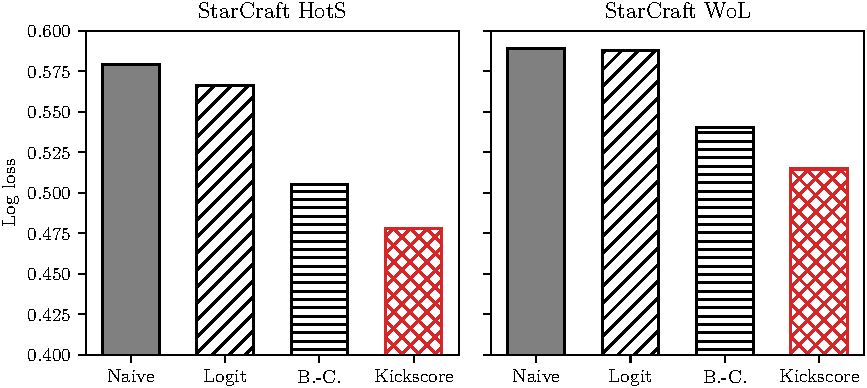
\includegraphics[width=\textwidth*3/4]{kks-starcraft}
	\caption{
		Average log loss of four models (Bradley--Terry, naive, blade-chest and ours) on the StarCraft datasets.}
	\label{kks:fig:starcraft}
\end{figure}


%%%%%%%%%%%%%%%%%%%%%%%%%%%%%%%%
\subsection{Inference Algorithm}
\label{kks:sec:evalinf}
We turn our attention to the inference algorithm and study the impact of several implementation choices.
We start by quantifying the impact of the mean-field assumption~\eqref{kks:eq:approxpost} and of the choice of variational objective on predictive performance.
Then, we demonstrate the scalability of the algorithm on the ChessBase dataset and measure the acceleration obtained by parallelizing the algorithm.


\subsubsection{Mean-Field Approximation}
In order to gain understanding on the impact of the factorization assumption in~\eqref{kks:eq:approxpost}, we devise the following experiment.
We consider a small subset of the basketball data containing all matches between 2000 and 2005 ($N = 6382$, $M = 32$).
We evaluate the predictive performance on each week of the last season by using all the matches prior to the test week as training data.
Our model uses a one-to-one mapping between teams and features, a constant + Matérn 1/2 covariance function, and a Gaussian likelihood on the points difference.

We compare the predictive performance resulting from two inference variants,
\begin{enuminline}
	\item mean-field approximate inference, \textit{i.e.}, Algorithm~\ref{alg:inference}, and
	\item \emph{exact} posterior inference\footnote{%
		This is possible for this particular choice of likelihood thanks to the self-conjugacy of the Gaussian distribution, but at a computational cost $O(N^3)$.}.
\end{enuminline}
Both approaches lead to an average log loss of \num{0.634} and an average accuracy of \num{0.664}.
Strikingly, both values are equal up to four decimal places, suggesting that the mean-field assumption is benign in practice~\citep{birlutiu2007expectation}.


\subsubsection{Variational Objective}
Next, we study the influence of the variational method.
We re-run the experiments of Section~\ref{kks:sec:evaldyn}, this time by using the reverse-KL objective instead of EP.
The predictive performance in terms of average log loss and average accuracy is equal to the EP case (Table~\ref{kks:tab:predperf}, last three columns) up to three decimal places, for all four datasets.
Hence, the variational objective seems to have little practical impact on predictive performance.
As such, we recommend using the reverse-KL objective for likelihoods whose log-partition function~\eqref{kks:eq:logpart} cannot be computed in closed form, as the numerical integration of the expected log-likelihood~\eqref{kks:eq:exp-ll} is generally more stable.


\subsubsection{Scalability}
Finally, we demonstrate the scalability of our inference algorithm by training a model on the full ChessBase dataset, containing over \num{7} million observations.
We implement a multithreaded version of Algorithm~\ref{alg:inference} in the Go programming language\footnote{%
	The code is available at \url{https://github.com/lucasmaystre/gokick}.}
and run the inference computation on a machine containing two 12-core Intel Xeon E5-2680 v3 (Haswell generation) processors clocked at 2.5 GHz.
Figure~\ref{kks:fig:scalability} displays the running time per iteration as function of the number of worker threads.
By using \num{16} threads, we need only slightly over \num{5} seconds per iteration.


\begin{figure}
	\centering
	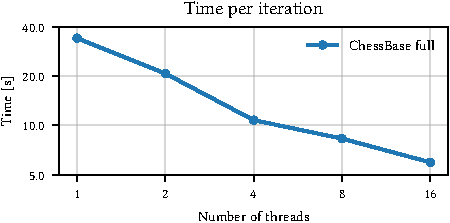
\includegraphics[width=\textwidth*3/4]{kks-scalability}
	\caption{
		Running time per iteration of a multithreaded implementation of Algorithm~\ref{alg:inference} on the ChessBase full dataset, containing over \num{7} million observations.}
	\label{kks:fig:scalability}
\end{figure}
